\chapter{Hasil Implementasi}
\label{appendix:hasil-implementasi}

Hasil implementasi sistem ini mencakup beberapa komponen utama yaitu komponen ekstraksi data pada gambar \ref{image:hasil-data-1}, sistem penyimpanan dan enrichment, antarmuka pengguna berbasis web pada gambar \ref{image:hasil-gui-1}, gambar \ref{image:hasil-gui-2}, gambar \ref{image:hasil-gui-3}, dan gambar \ref{image:hasil-gui-4}, serta antarmuka pengguna berbasis API pada gambar \ref{image:hasil-api-1}, gambar \ref{image:hasil-api-2}, dan gambar \ref{image:hasil-api-3}.

\begin{figure}[ht]
	\centering
	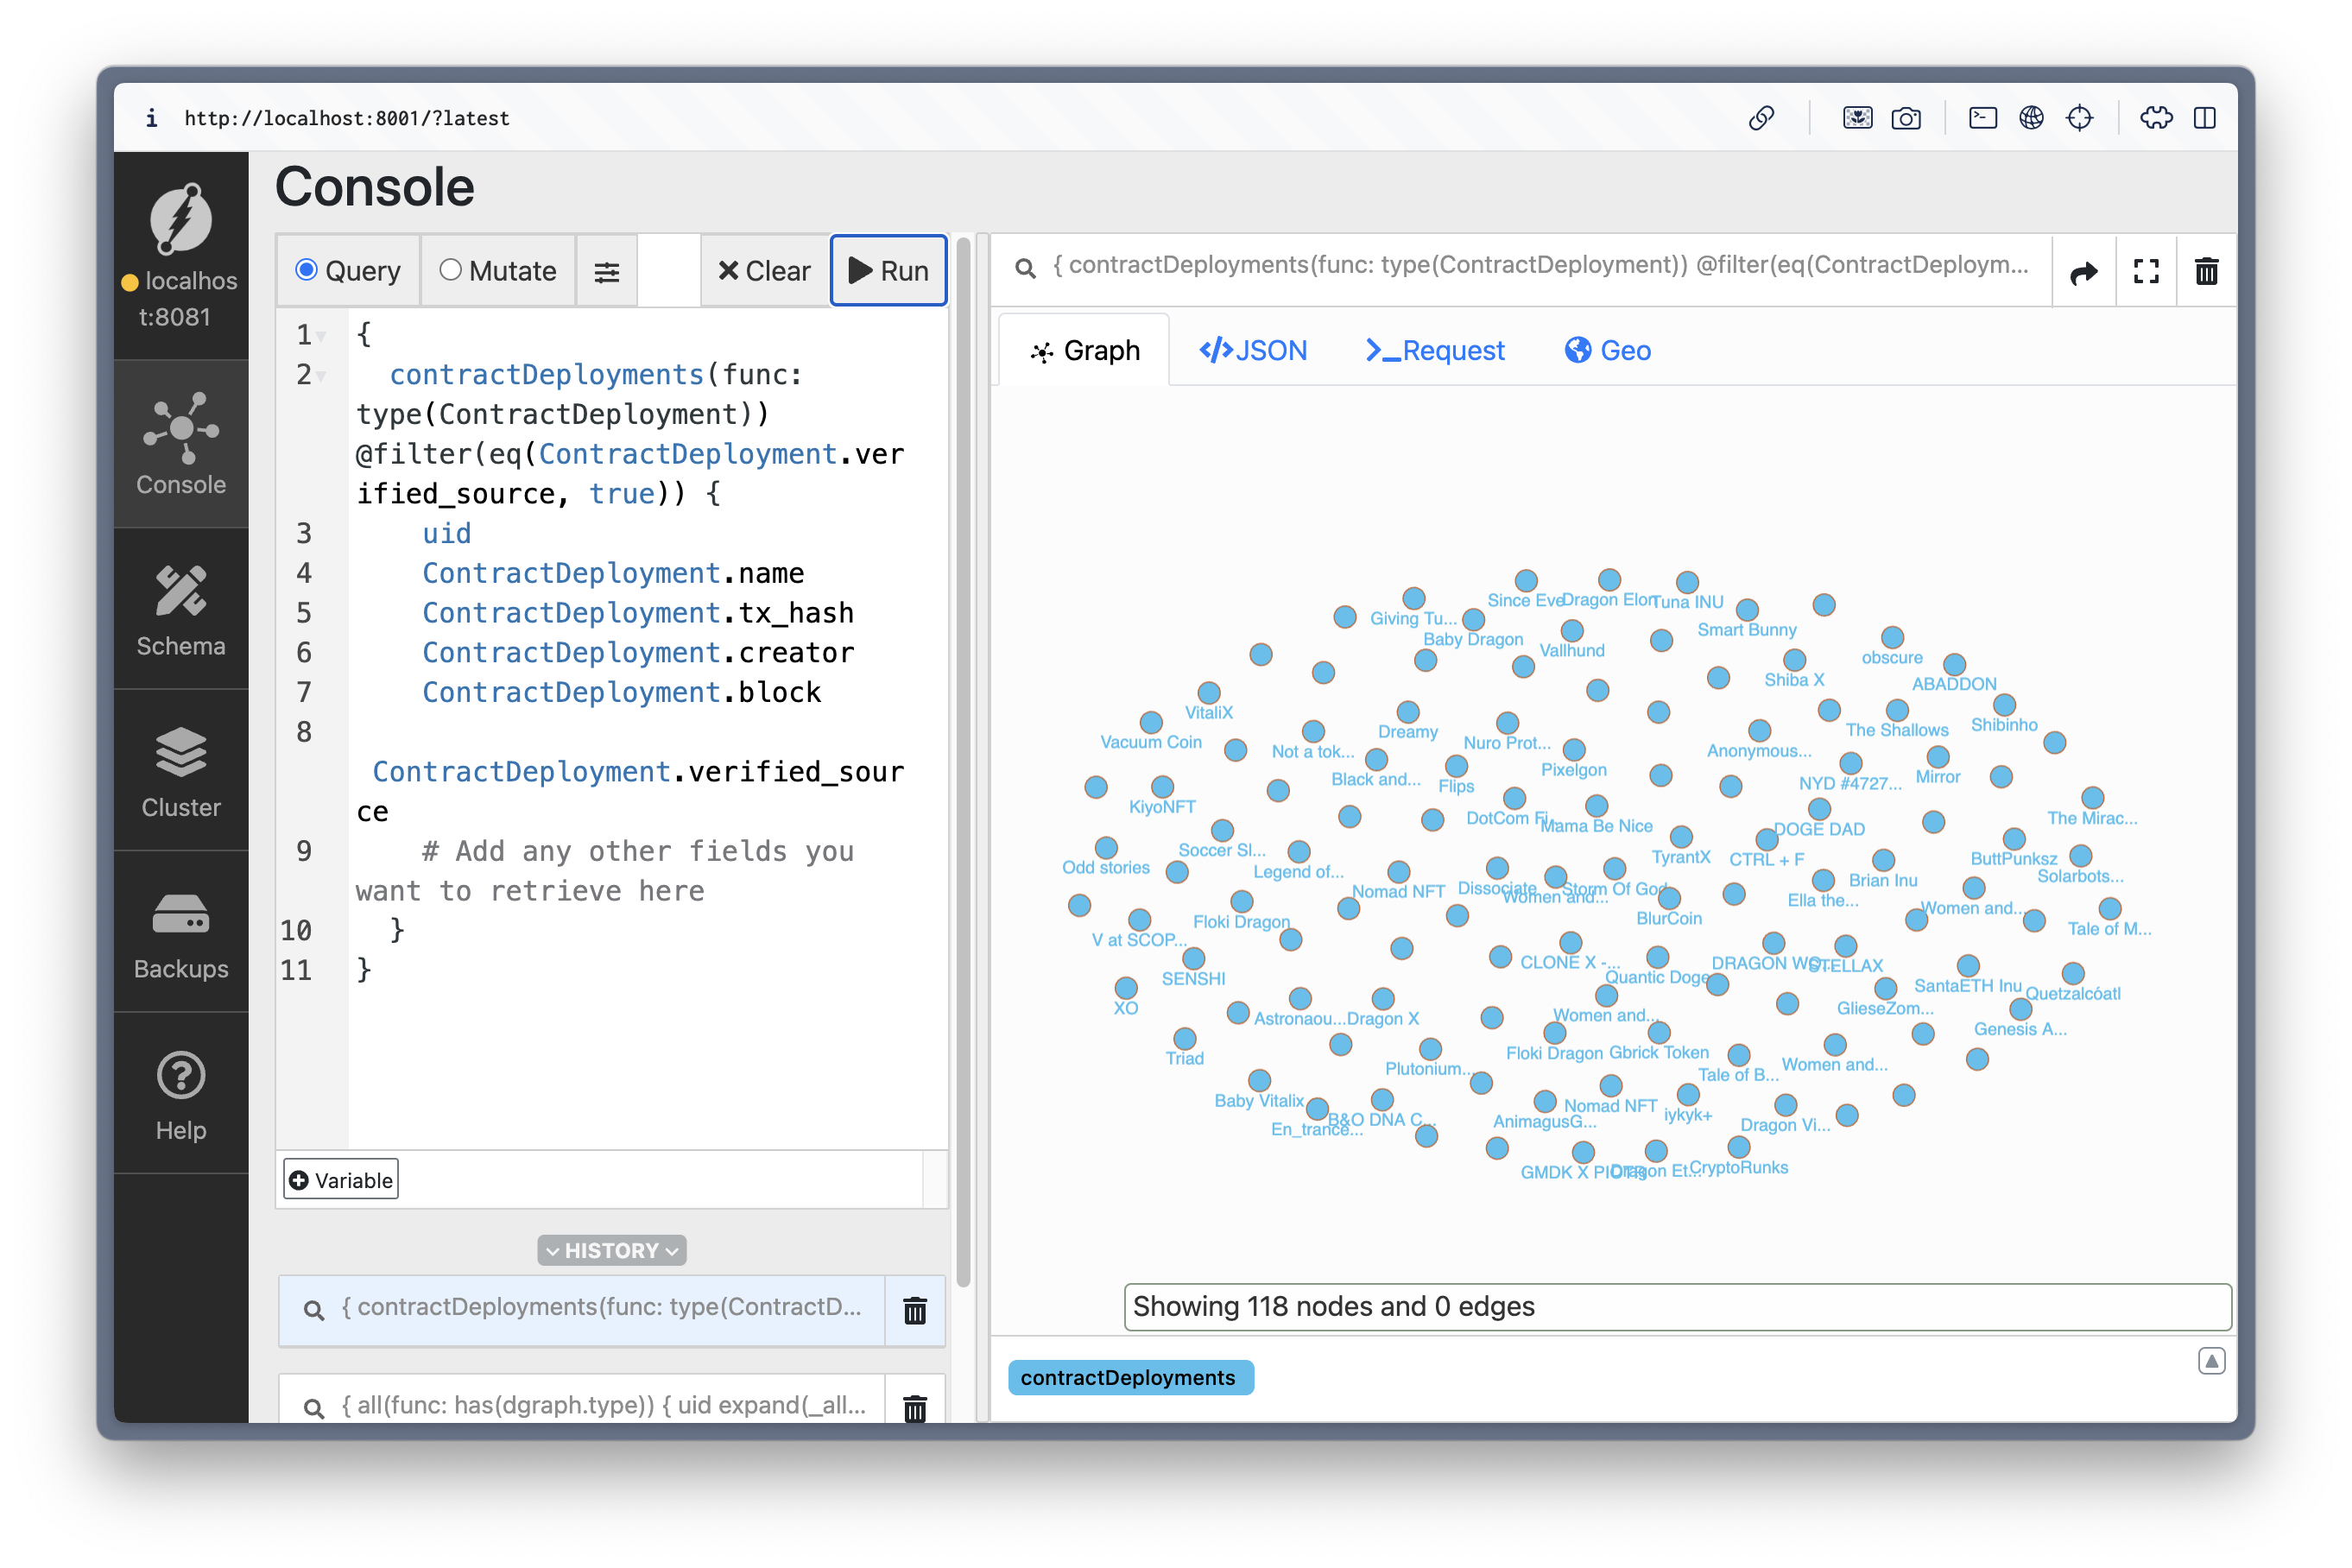
\includegraphics[width=1\textwidth]{resources/appendix/hasil-data-1.png}
	\caption{Hasil ekstraksi data}
	\label{image:hasil-data-1}
\end{figure}

\begin{figure}[ht]
	\centering
	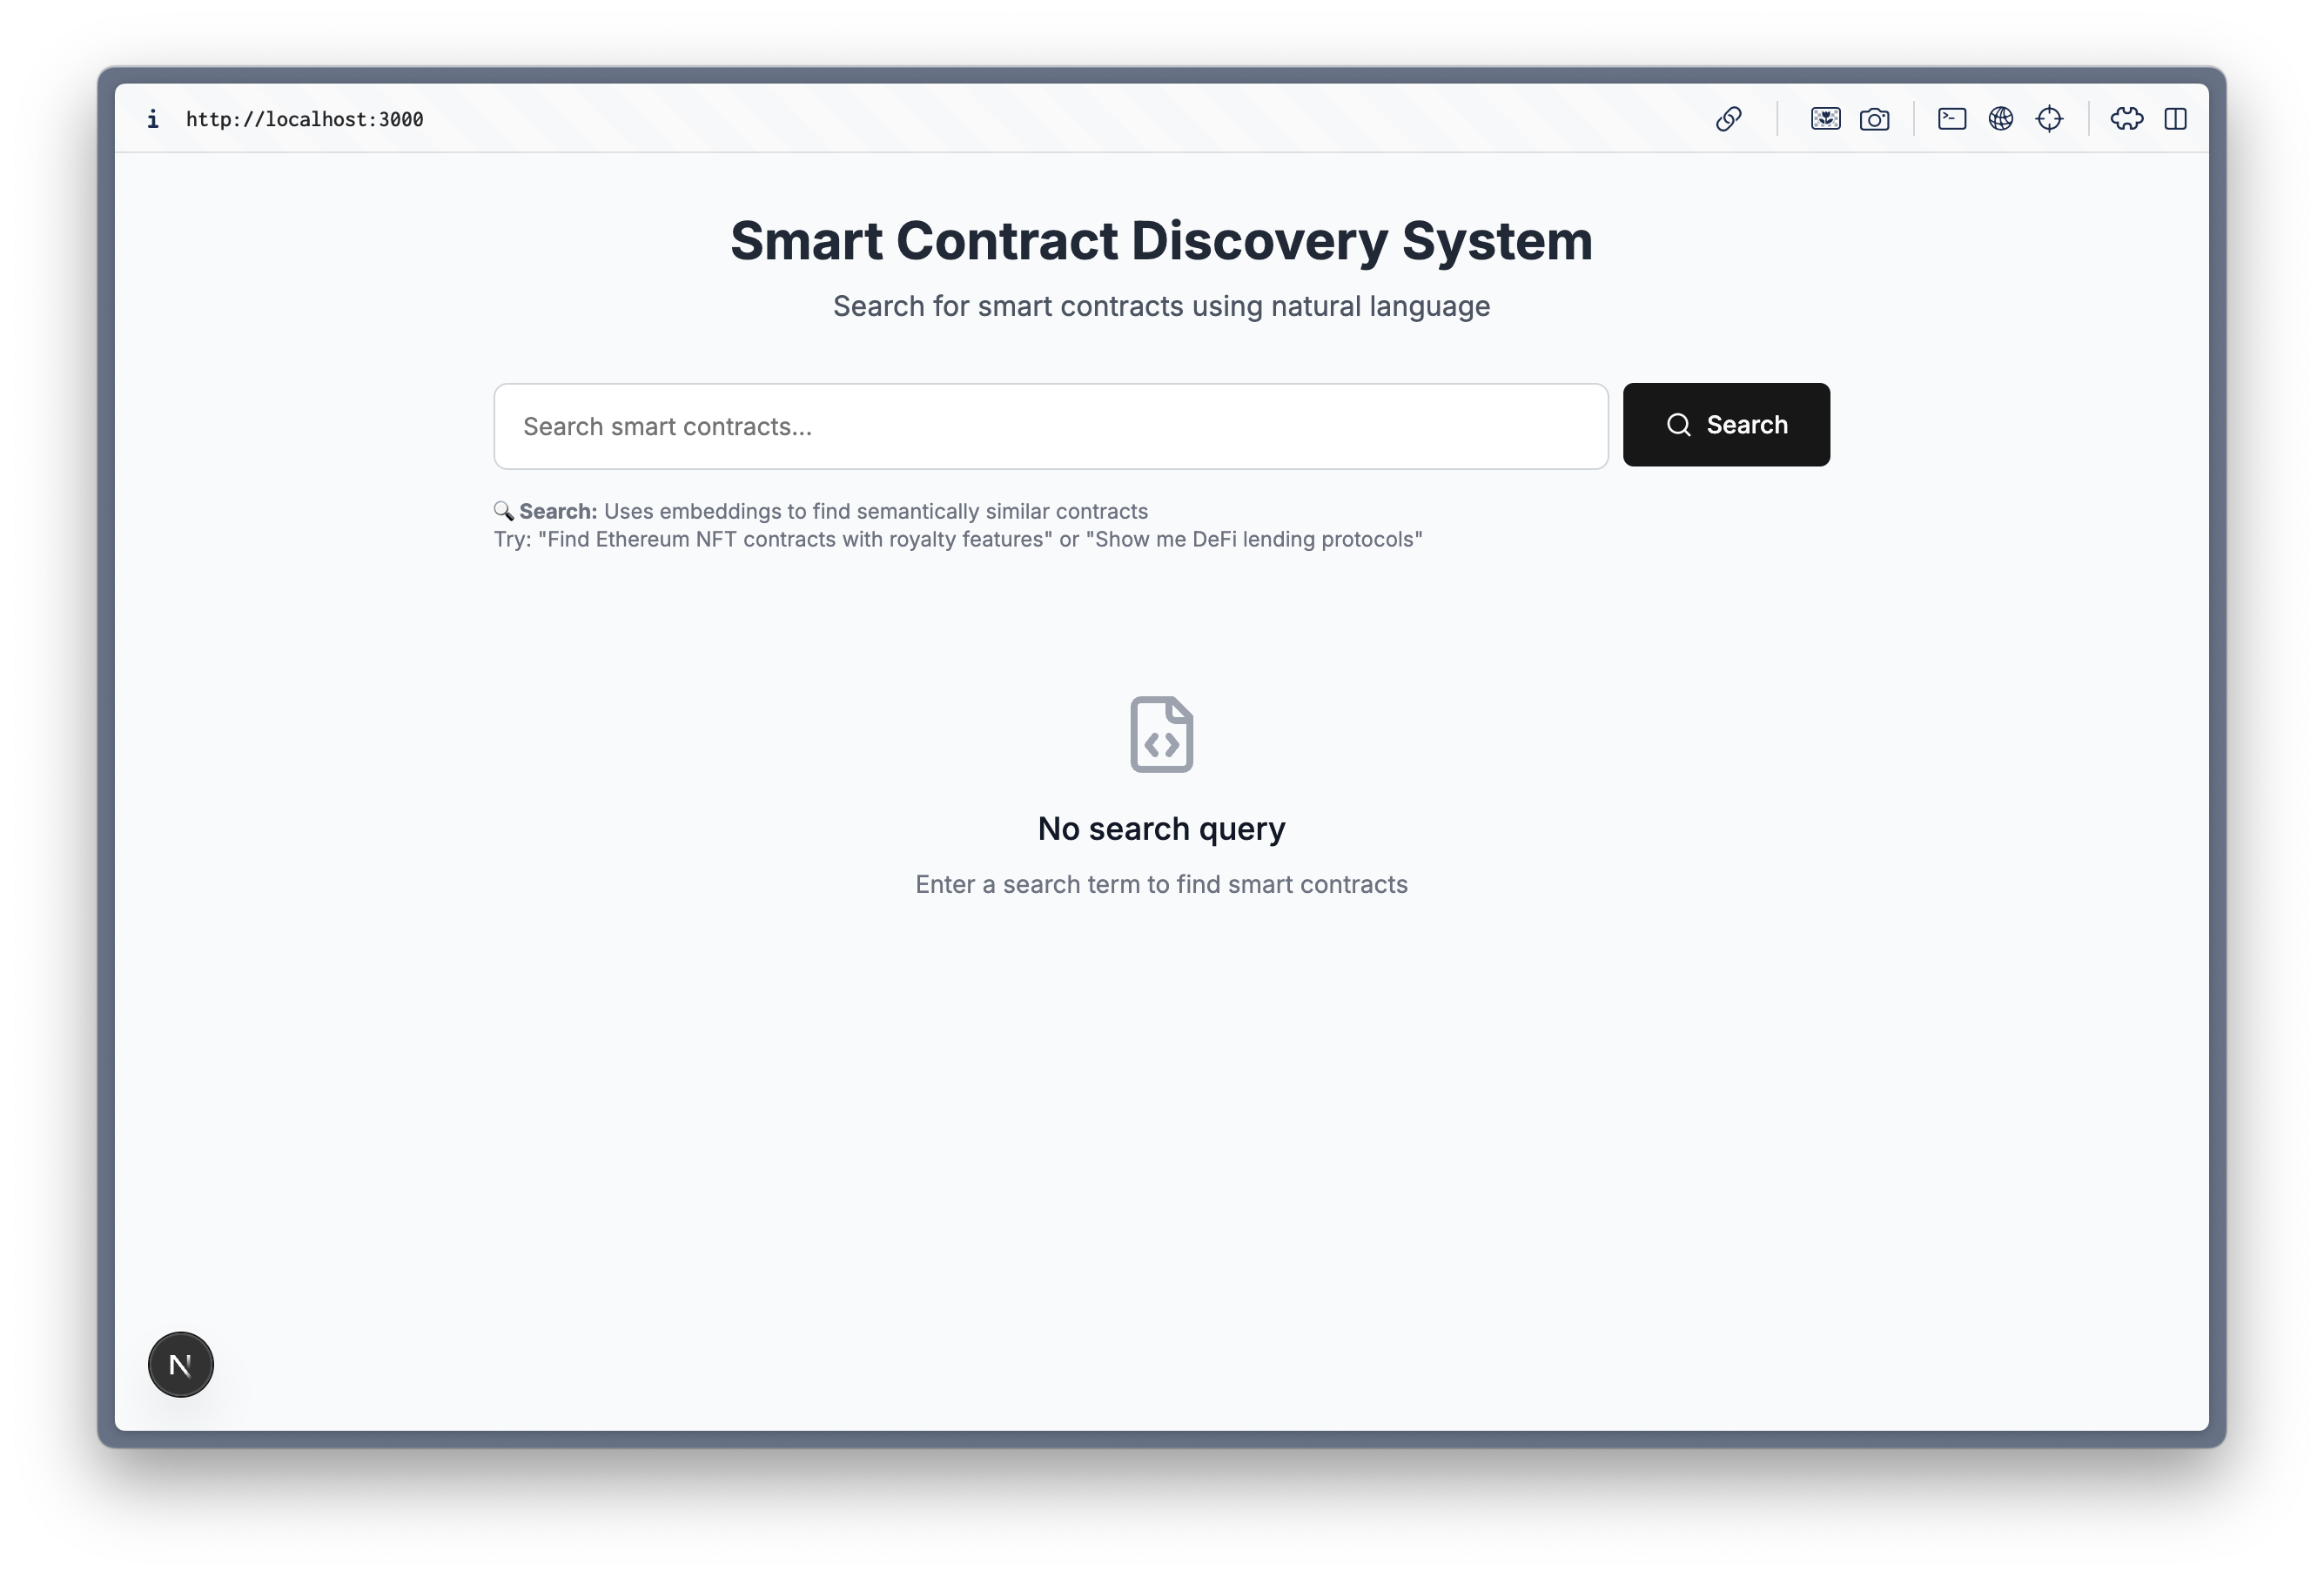
\includegraphics[width=1\textwidth]{resources/appendix/hasil-gui-1.png}
	\caption{Hasil antarmuka pengguna}
	\label{image:hasil-gui-1}
\end{figure}

\begin{figure}[ht]
	\centering
	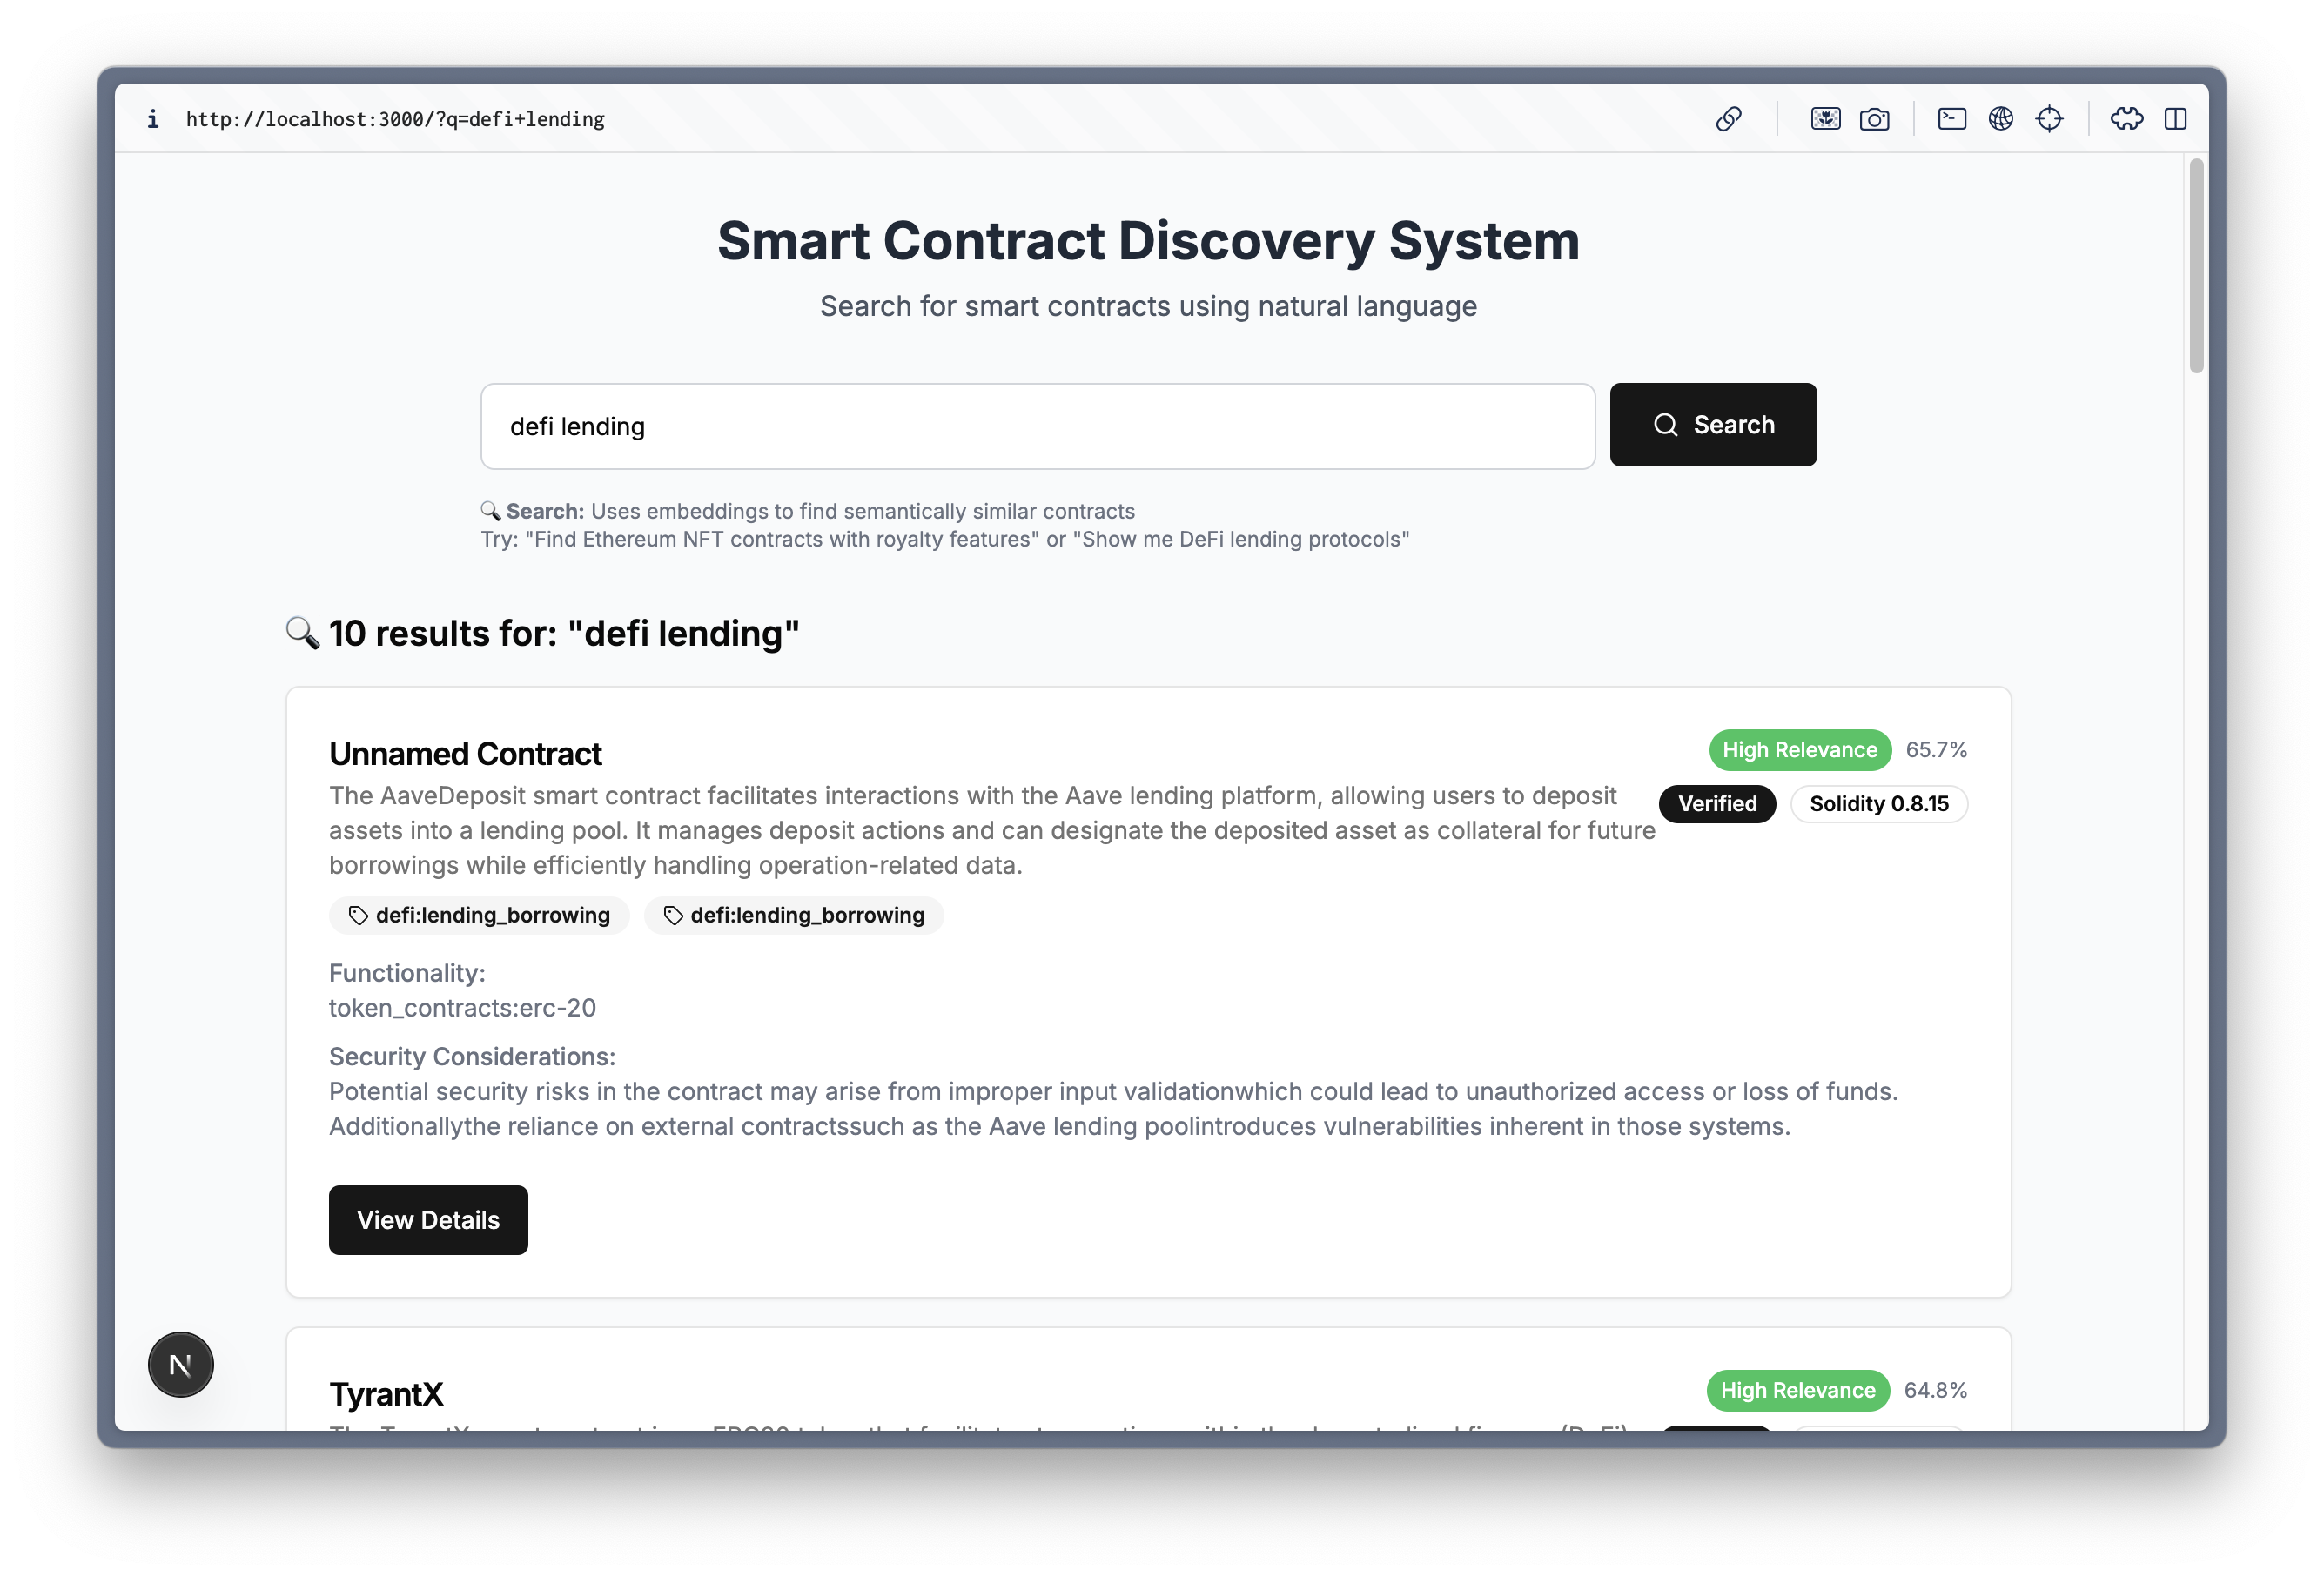
\includegraphics[width=1\textwidth]{resources/appendix/hasil-gui-2.png}
	\caption{Hasil antarmuka pengguna}
	\label{image:hasil-gui-2}
\end{figure}

\begin{figure}[ht]
	\centering
	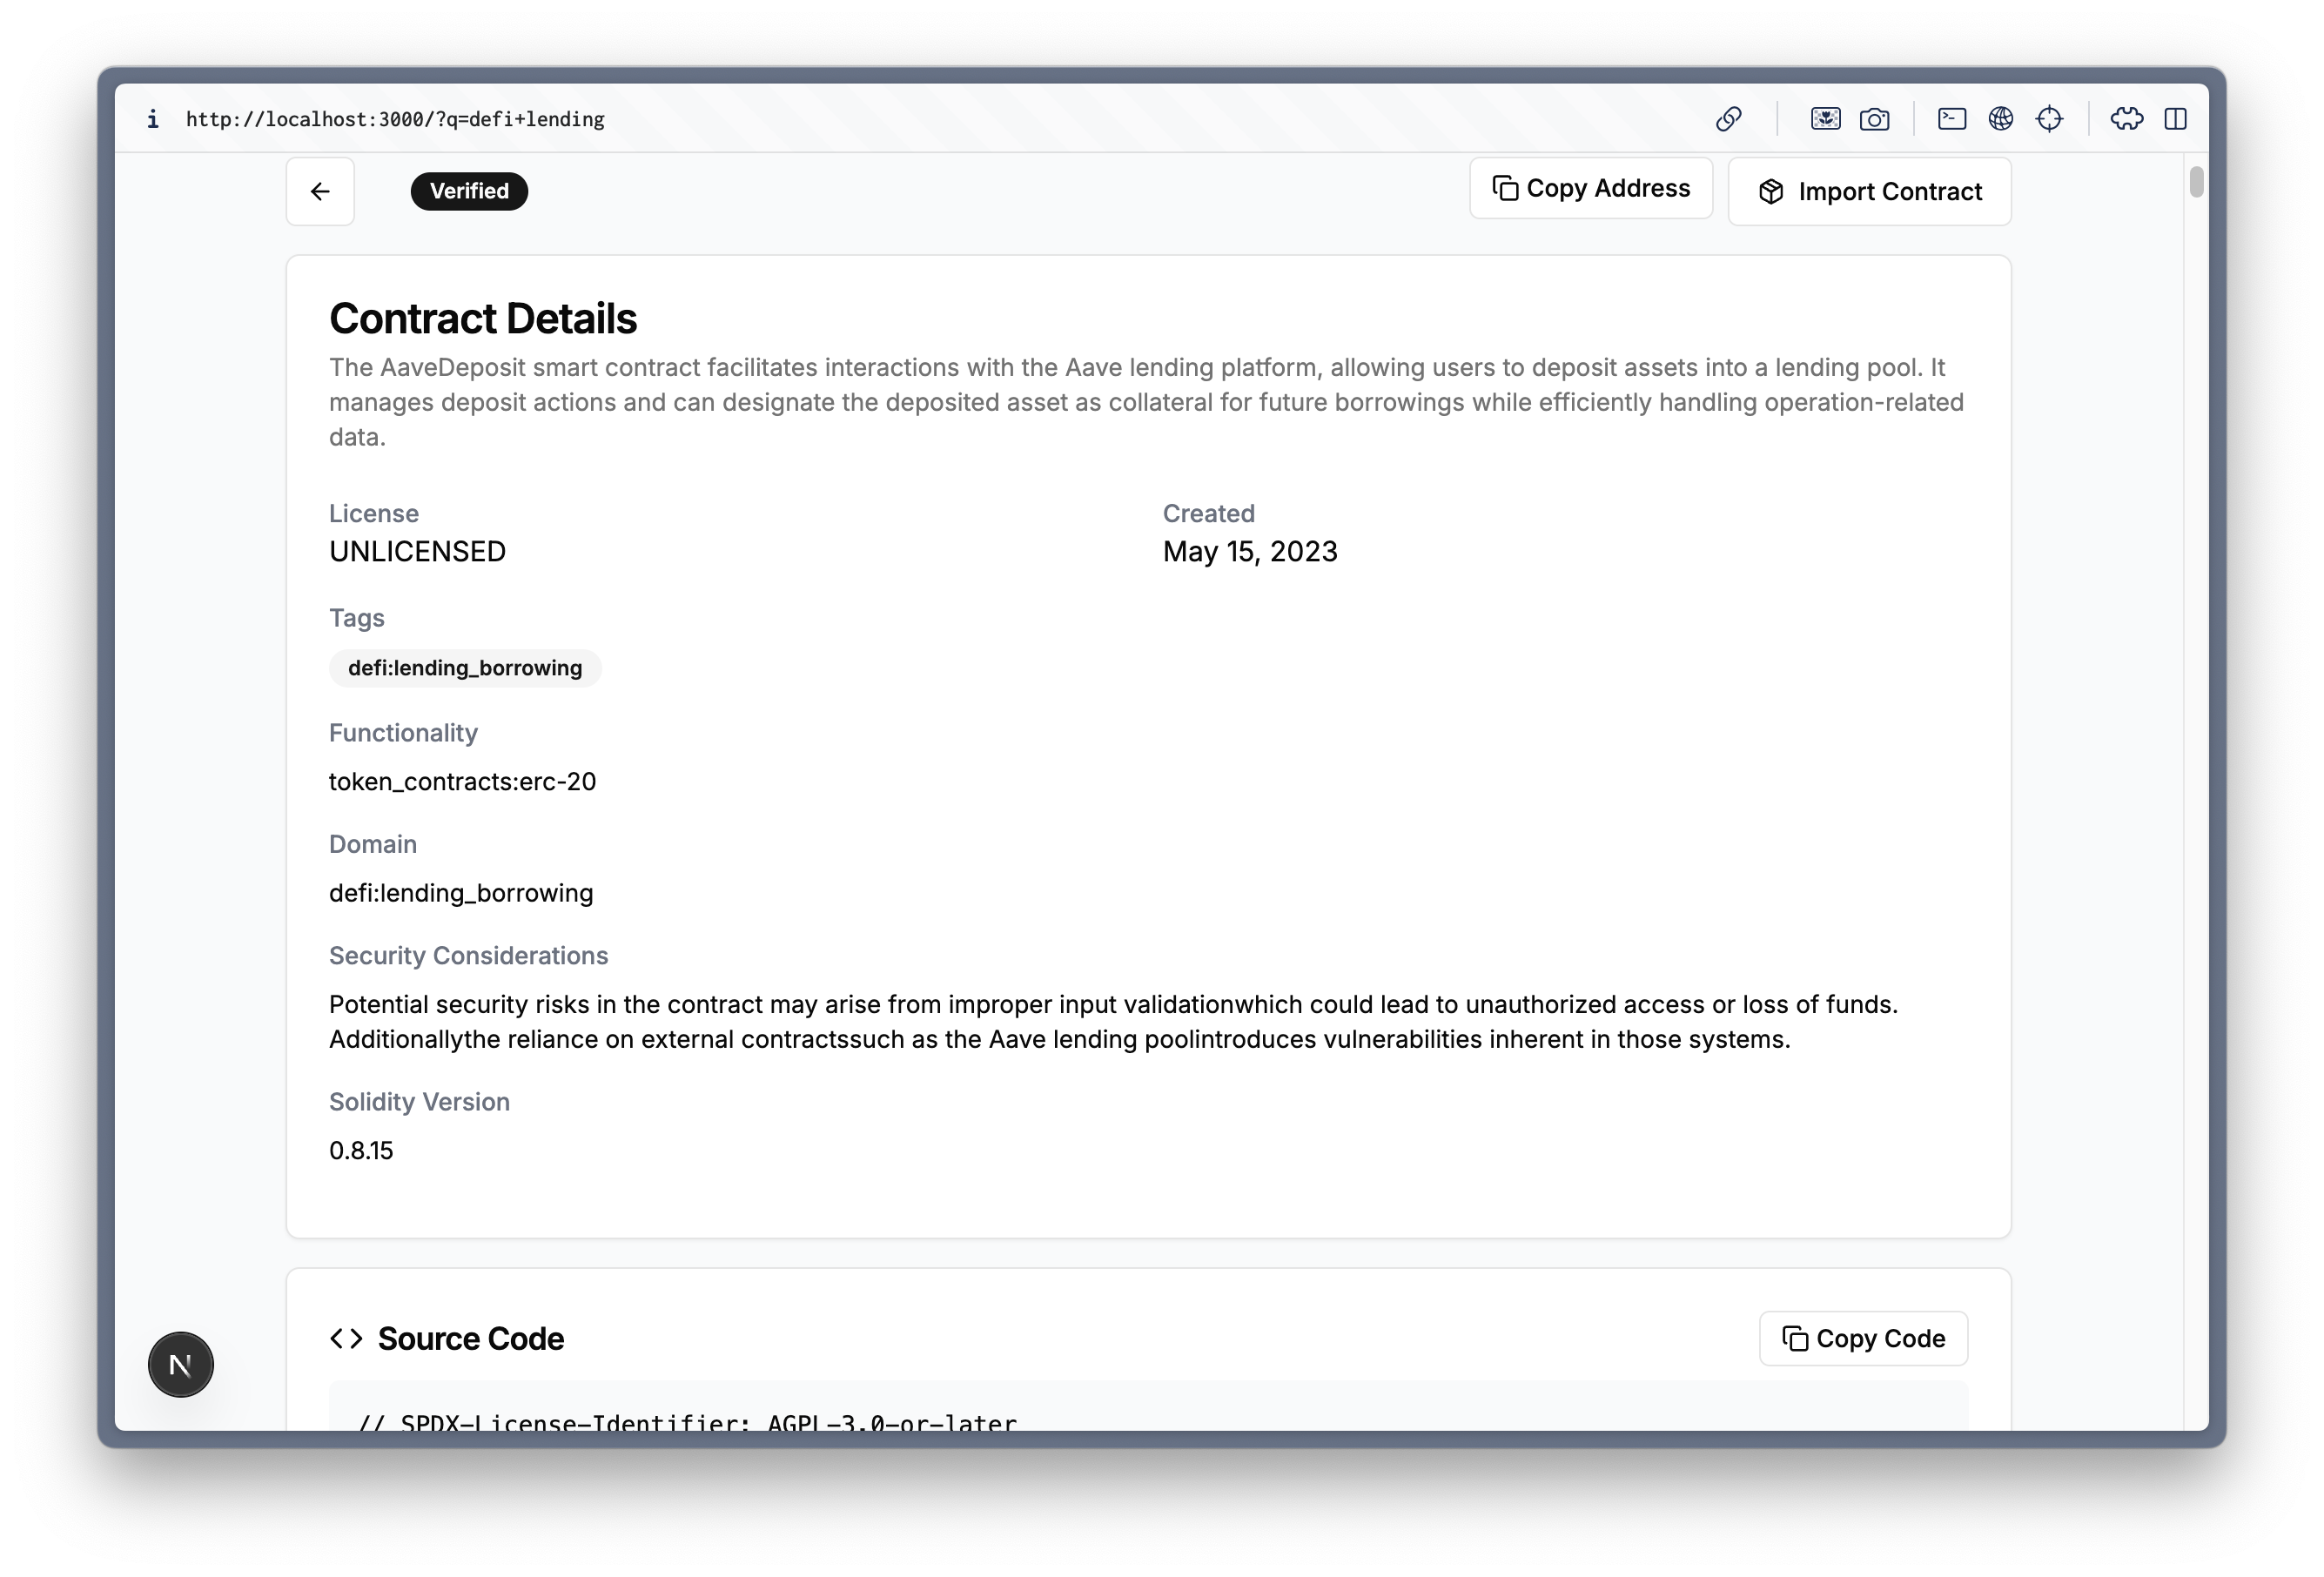
\includegraphics[width=1\textwidth]{resources/appendix/hasil-gui-3.png}
	\caption{Hasil antarmuka pengguna}
	\label{image:hasil-gui-3}
\end{figure}

\begin{figure}[ht]
	\centering
	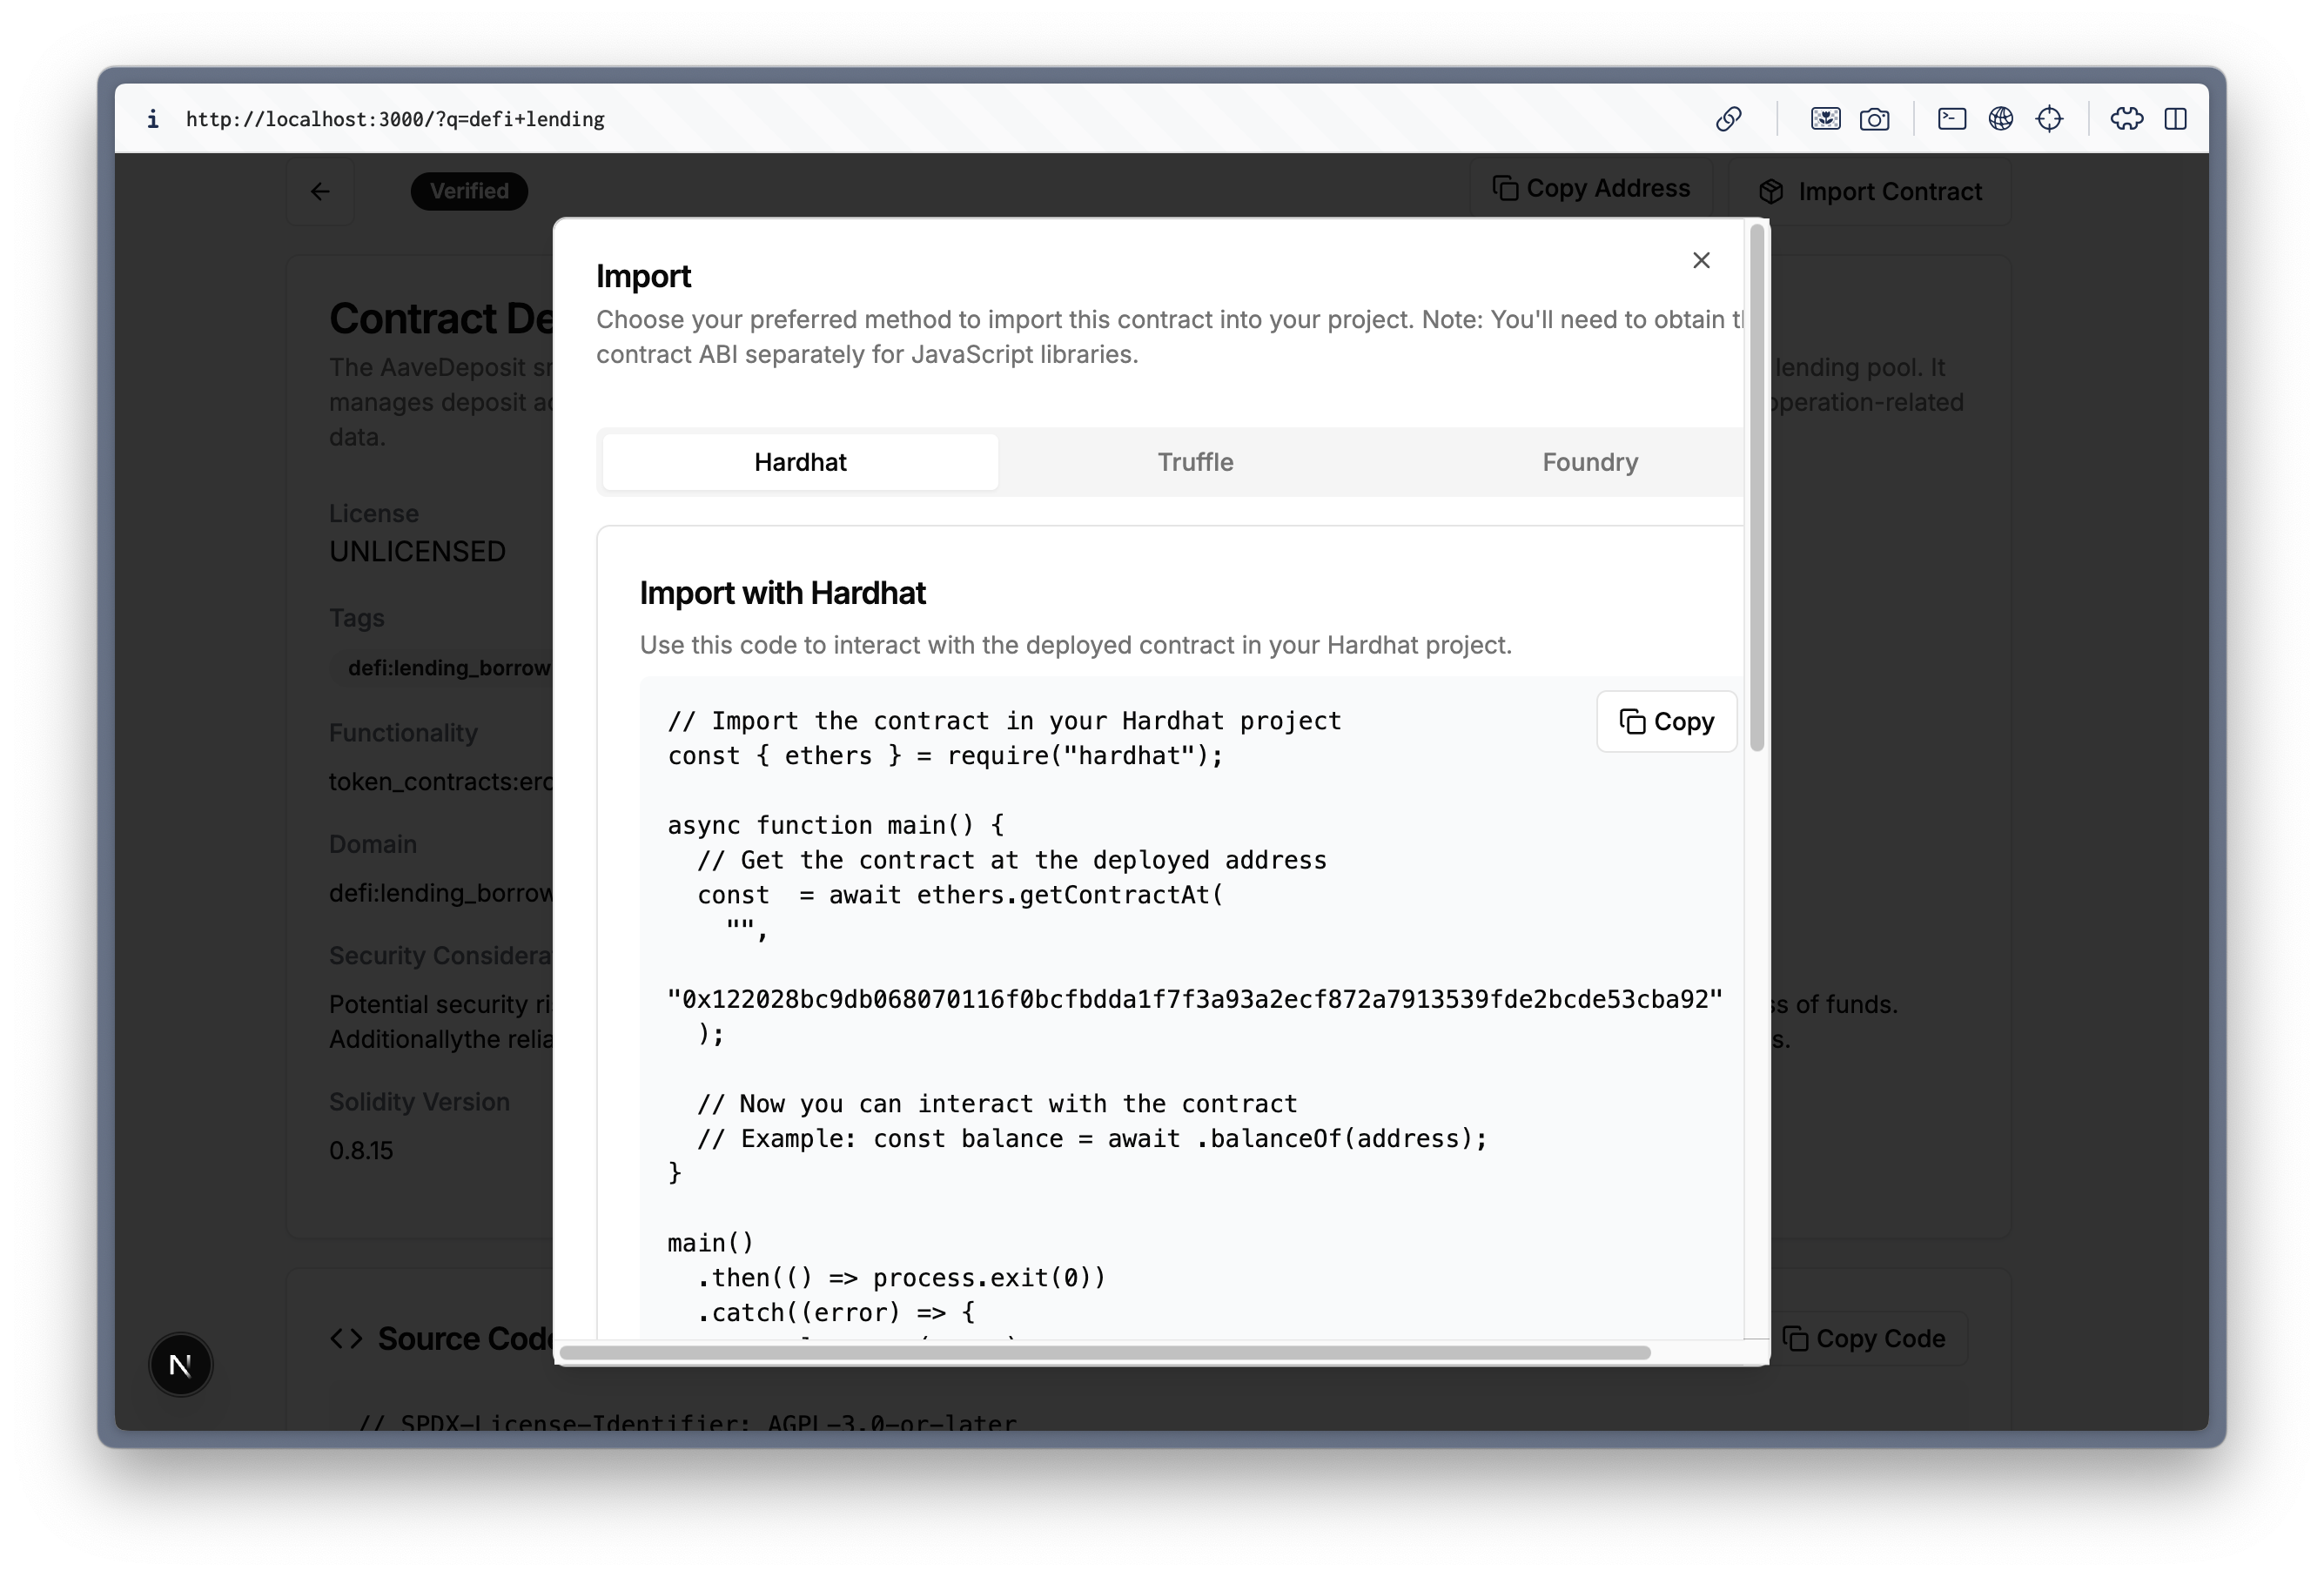
\includegraphics[width=1\textwidth]{resources/appendix/hasil-gui-4.png}
	\caption{Hasil antarmuka pengguna}
	\label{image:hasil-gui-4}
\end{figure}

\begin{figure}[ht]
	\centering
	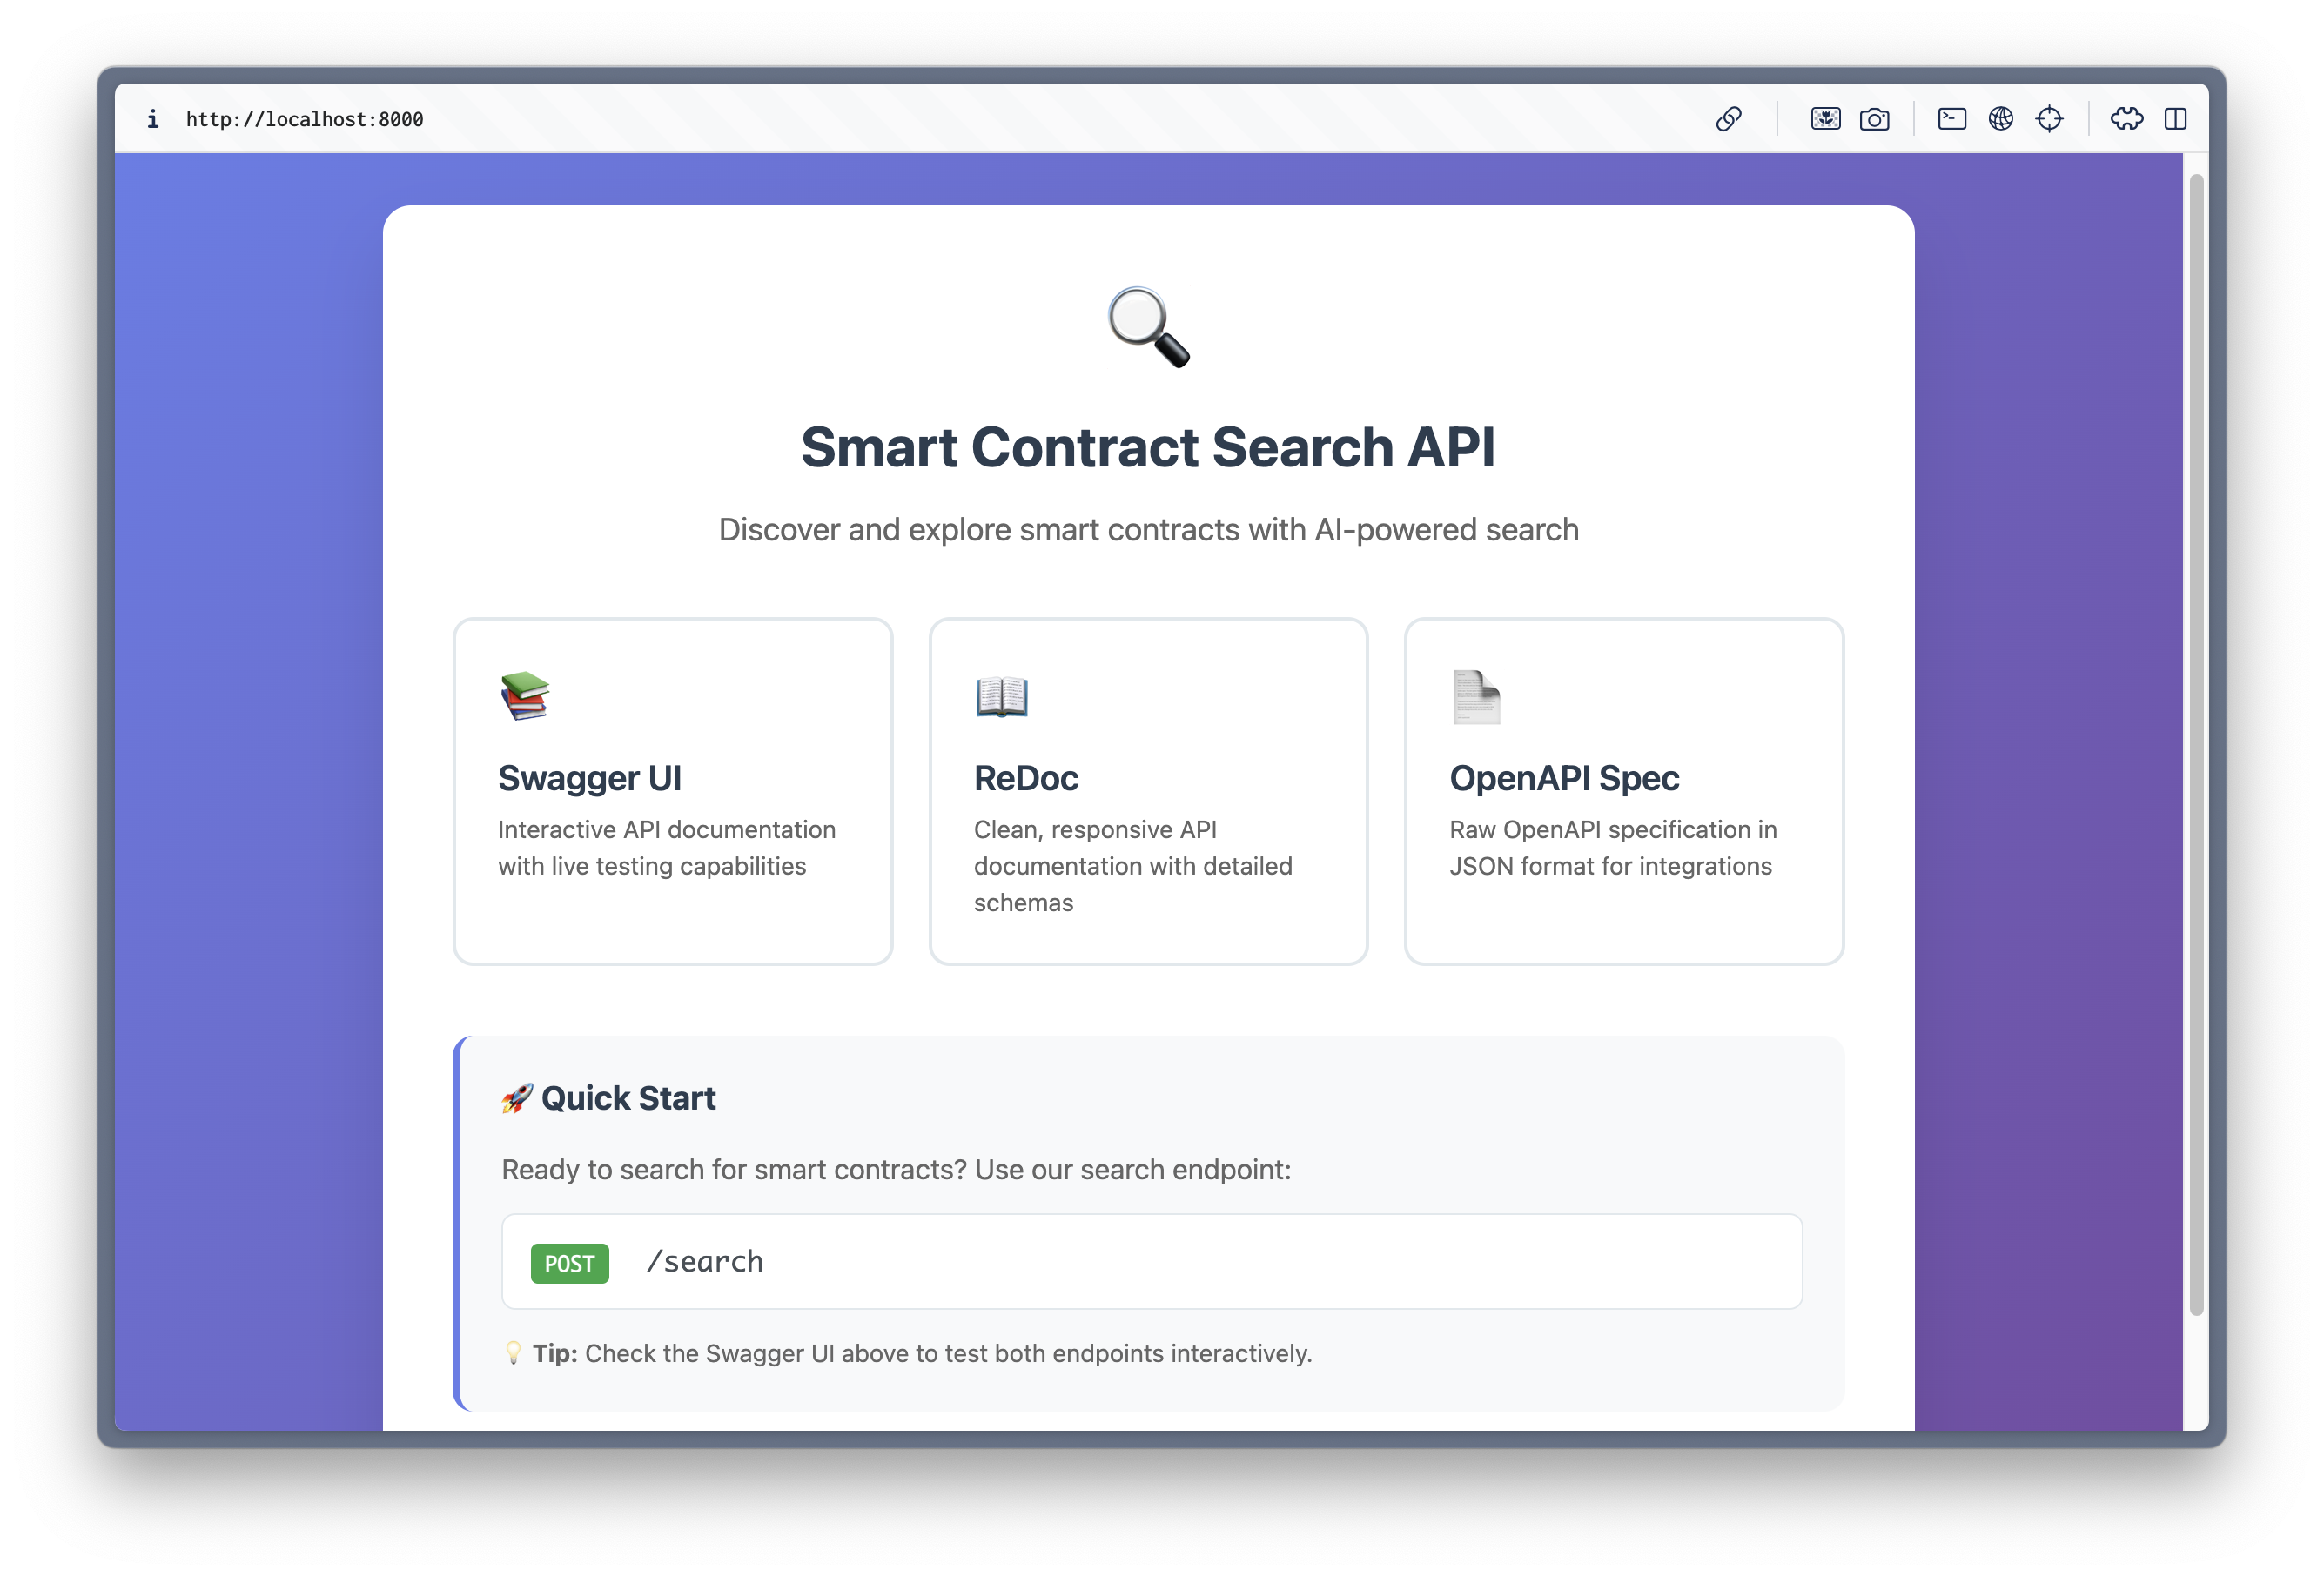
\includegraphics[width=1\textwidth]{resources/appendix/hasil-api-1.png}
	\caption{Hasil antarmuka pengguna}
	\label{image:hasil-api-1}
\end{figure}

\begin{figure}[ht]
	\centering
	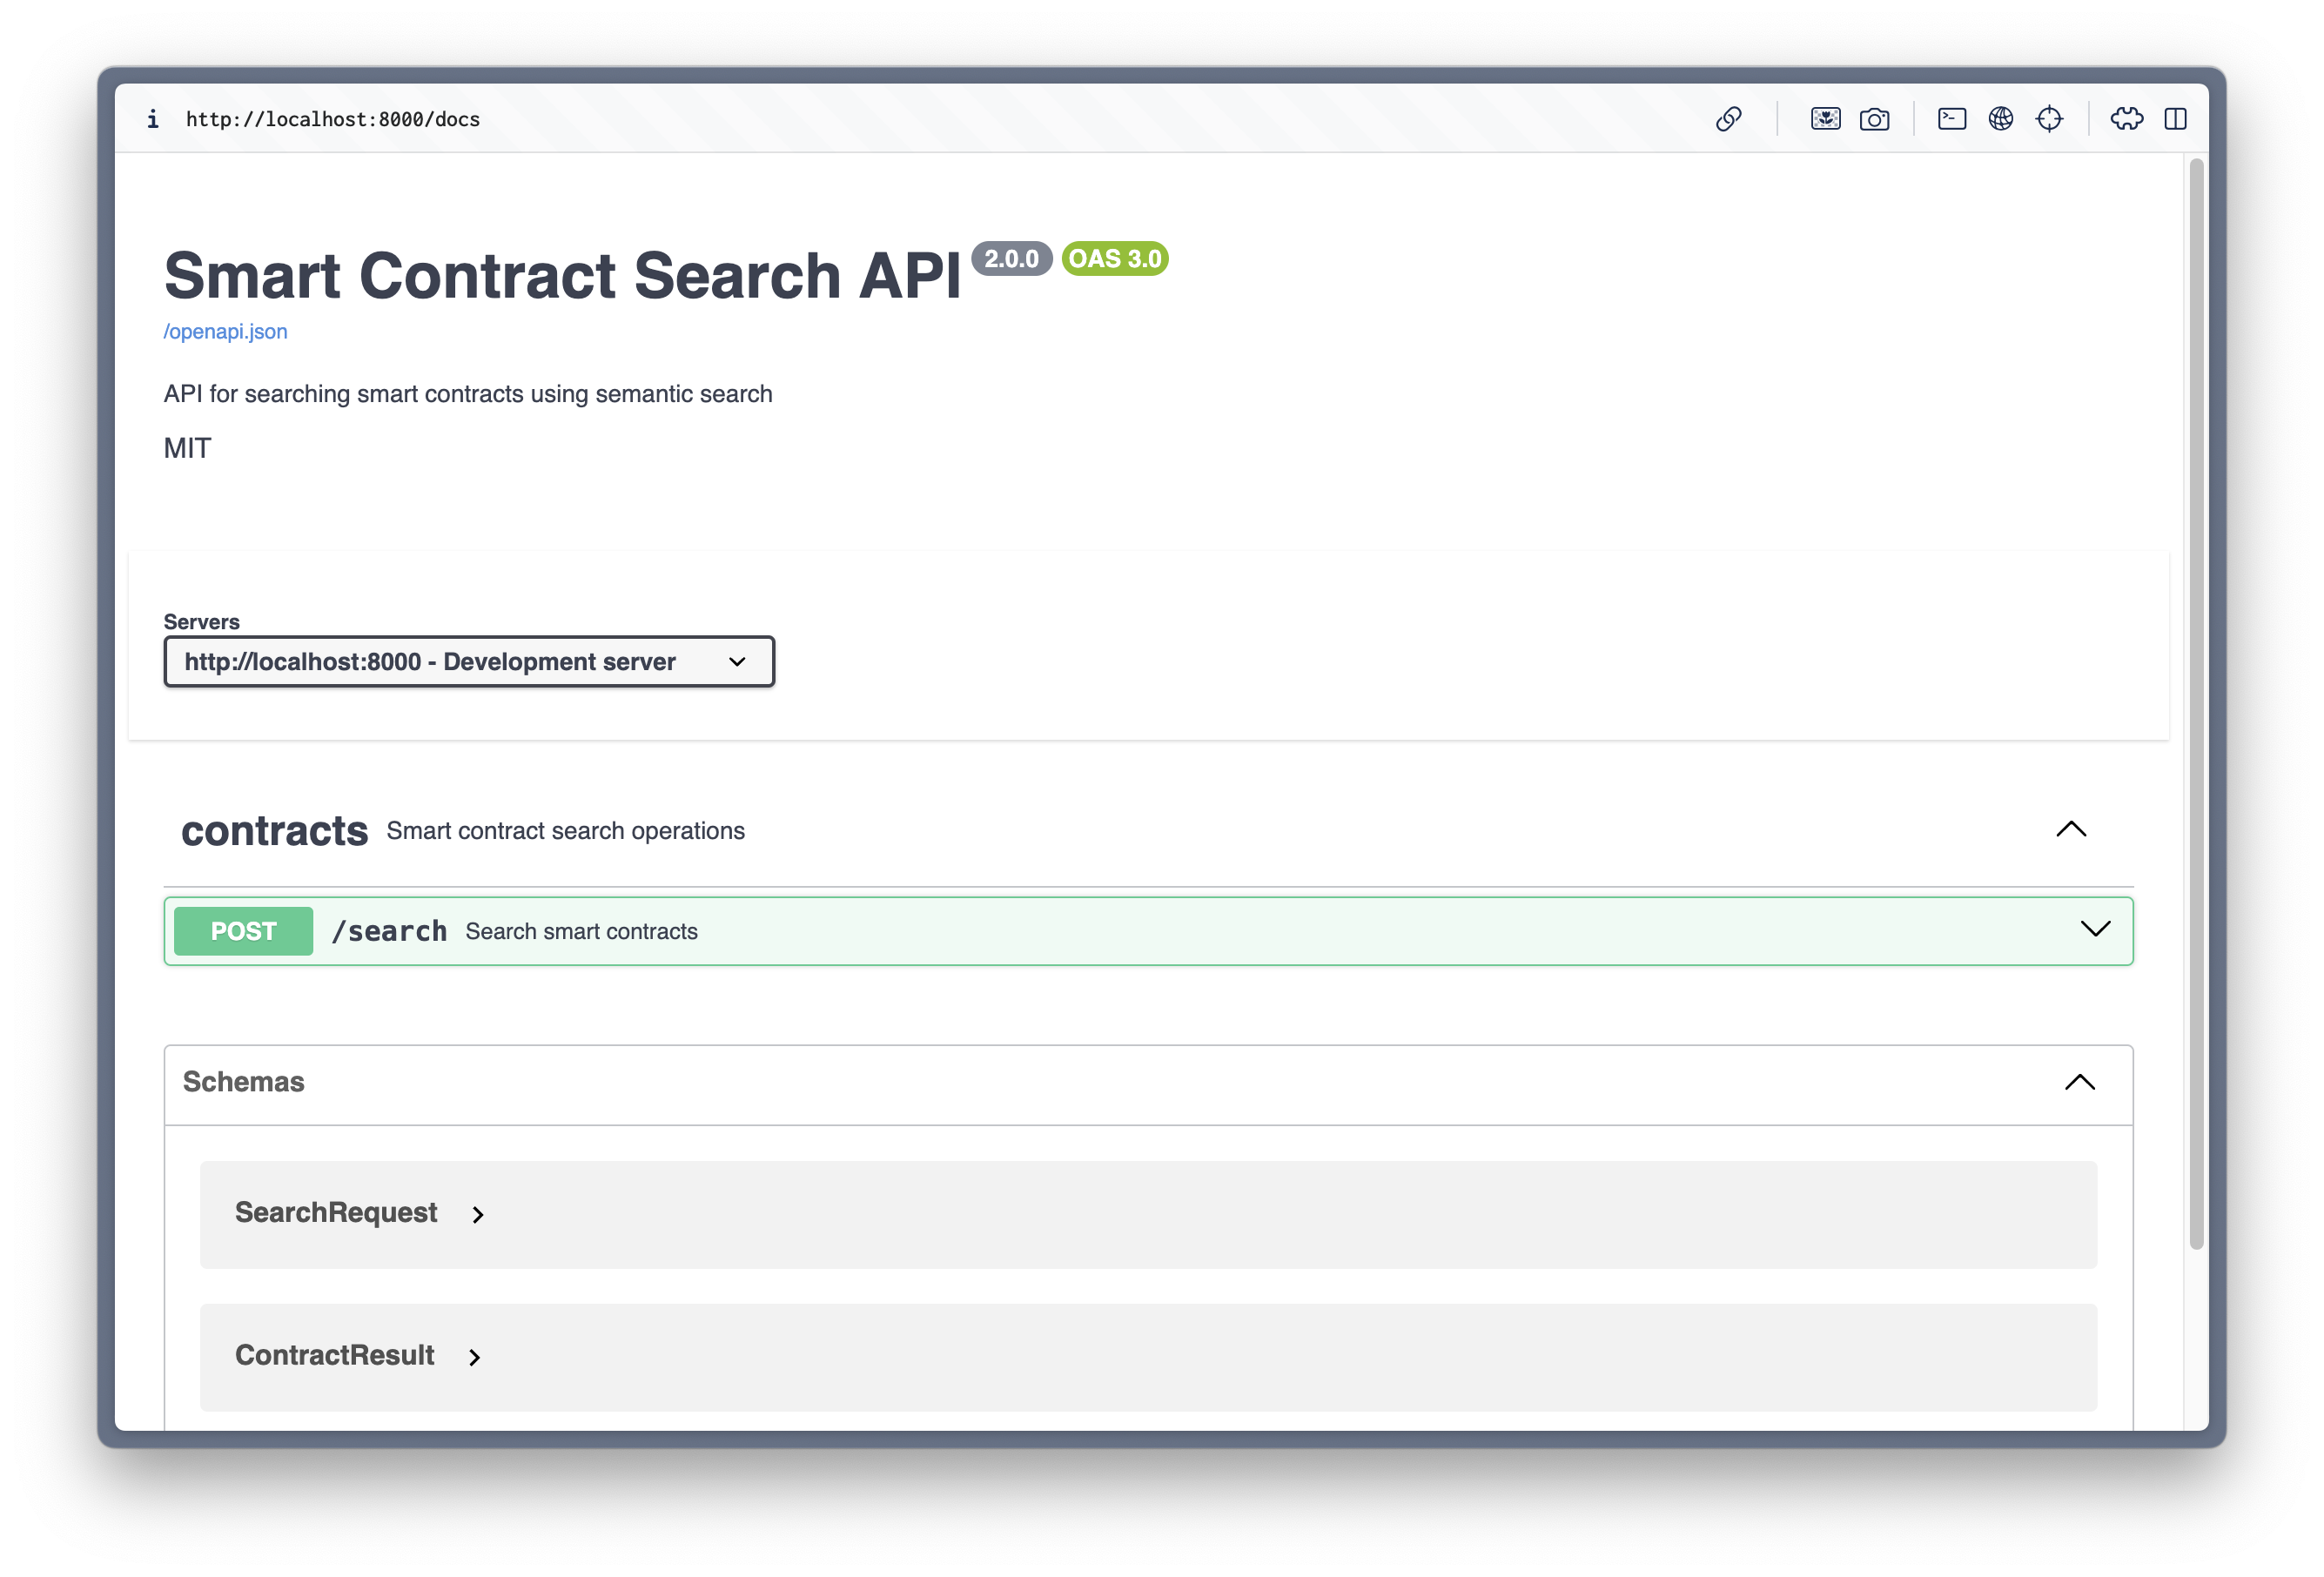
\includegraphics[width=1\textwidth]{resources/appendix/hasil-api-2.png}
	\caption{Hasil antarmuka pengguna}
	\label{image:hasil-api-2}
\end{figure}

\begin{figure}[ht]
	\centering
	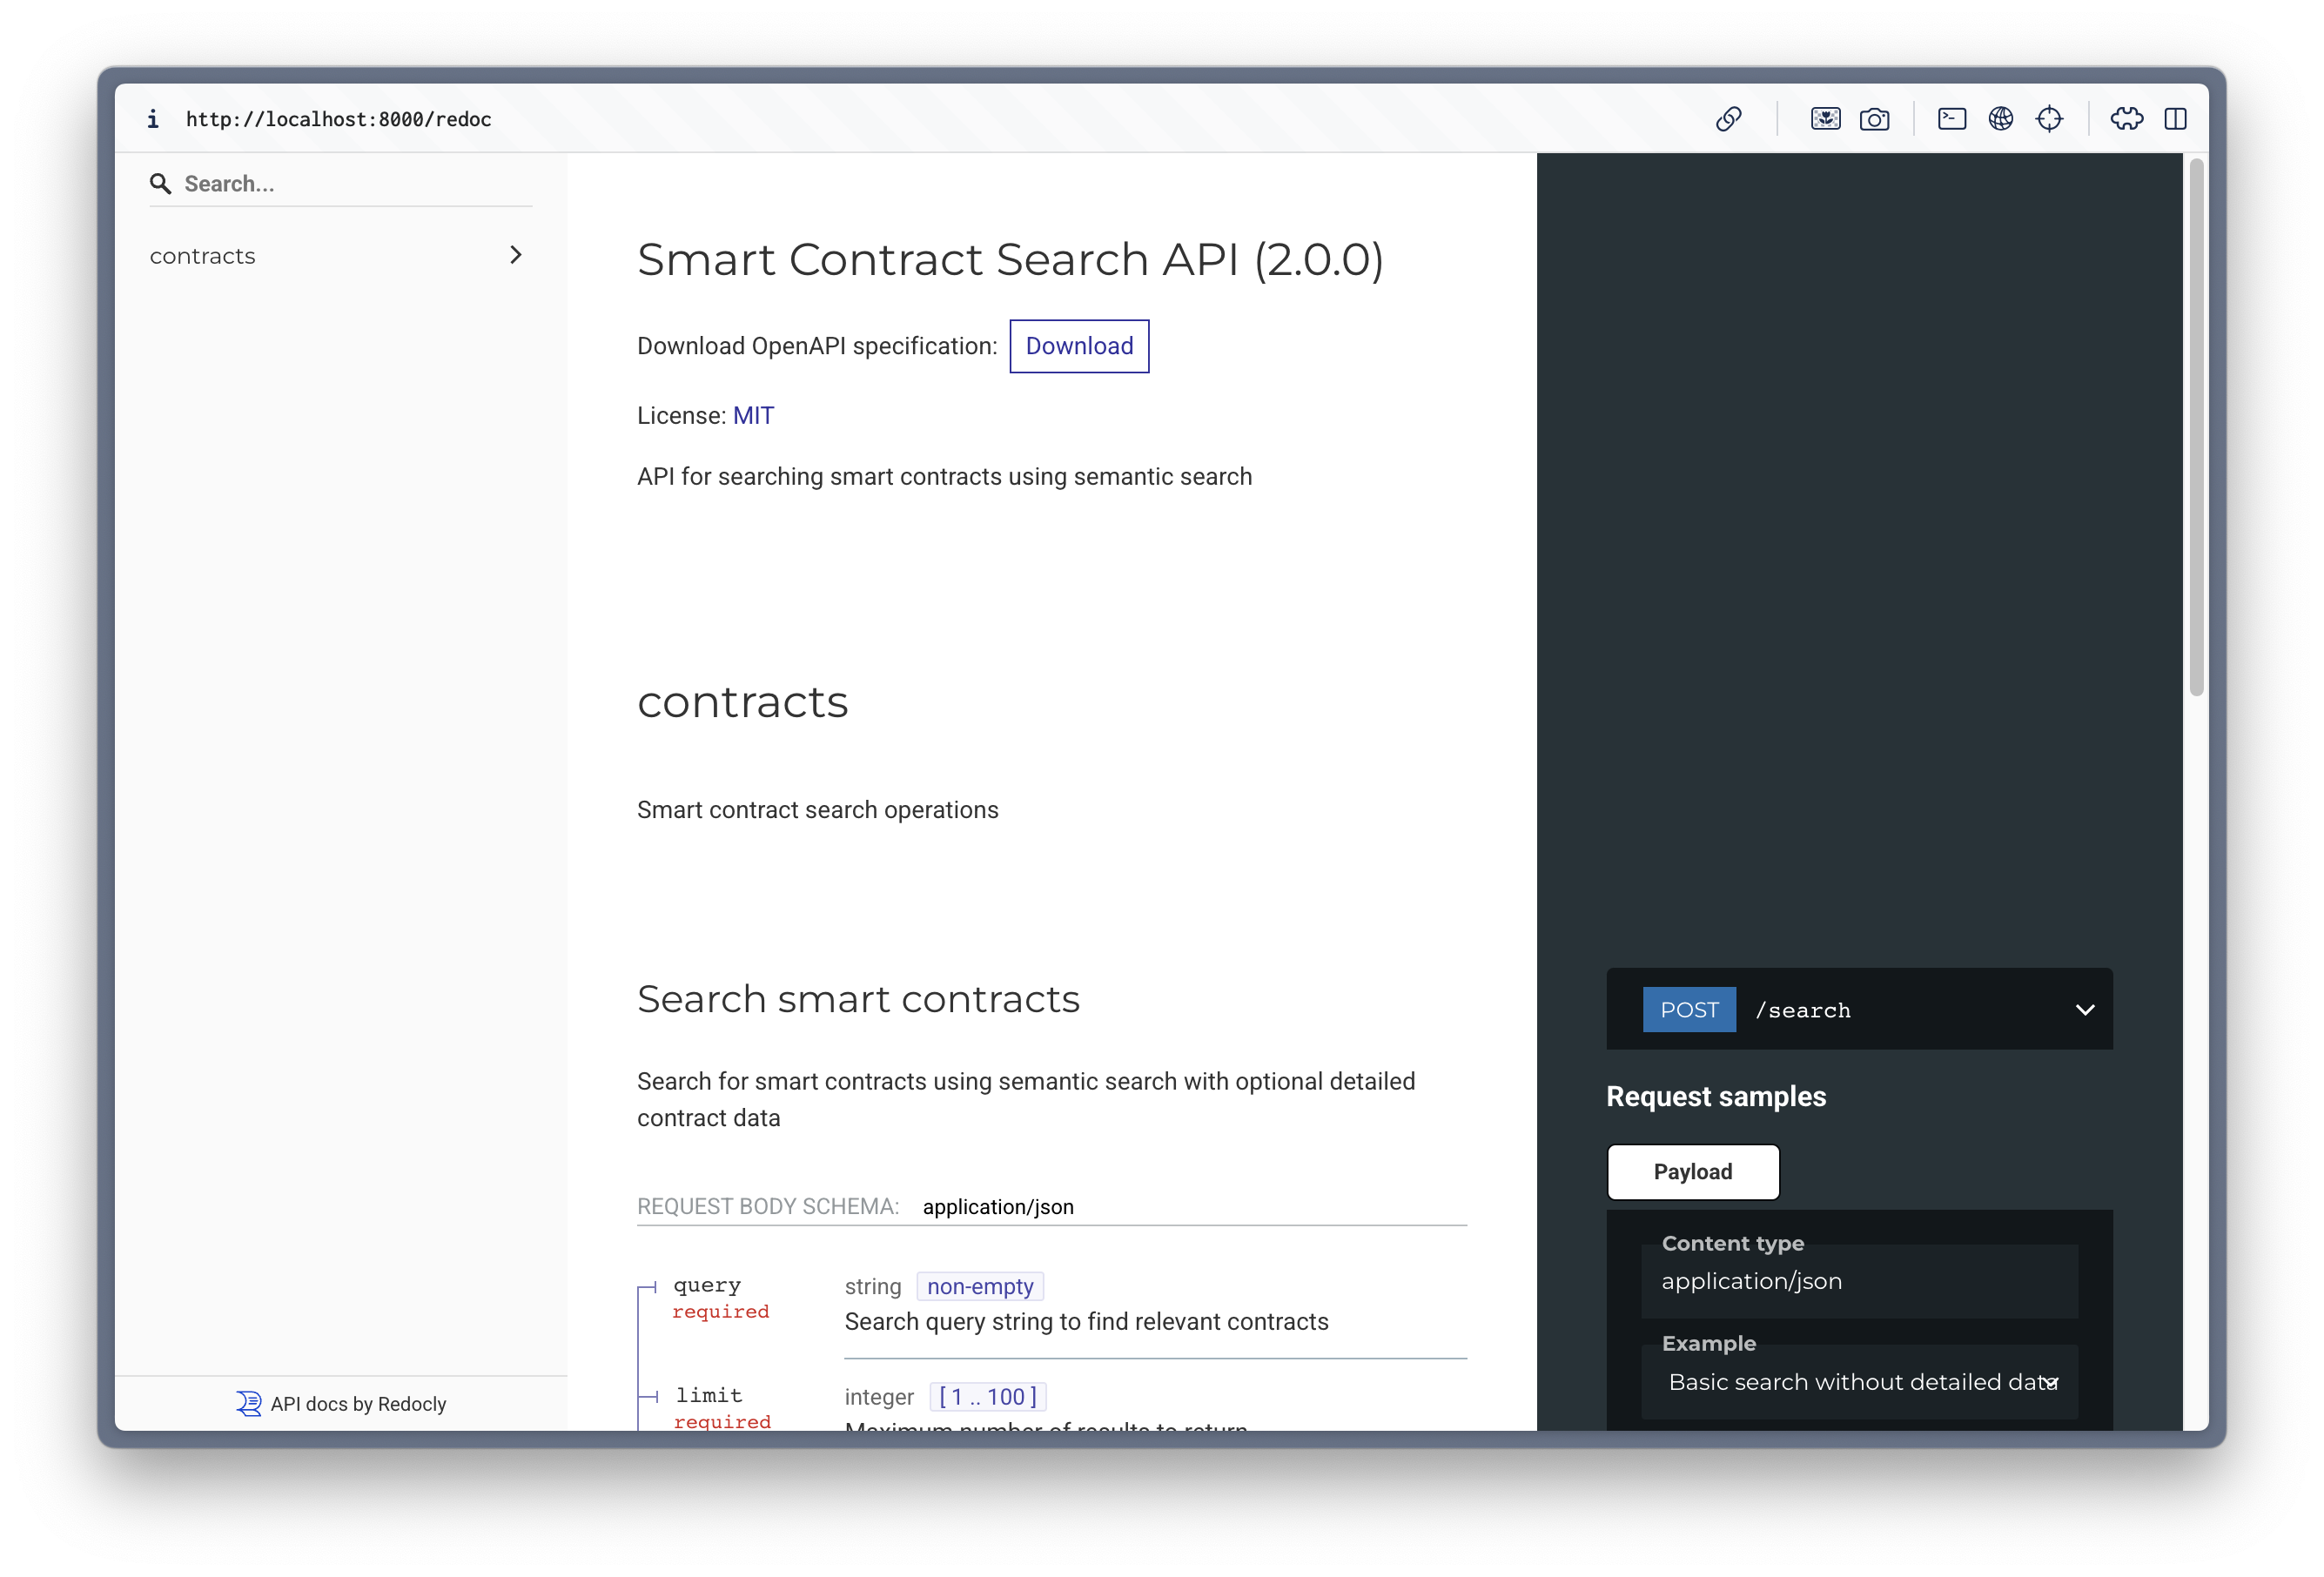
\includegraphics[width=1\textwidth]{resources/appendix/hasil-api-3.png}
	\caption{Hasil antarmuka pengguna}
	\label{image:hasil-api-3}
\end{figure}
